\documentclass[review]{elsarticle}

\usepackage[utf8]{inputenc}
\usepackage{lineno,hyperref}

\usepackage{color}
\usepackage{amsmath} % separar equação
%\usepackage[miktex,subfolder,cleanup]{gnuplottex} % Gnuplot
\usepackage{algorithmic}
\usepackage[ruled,lined,noend,linesnumbered]{algorithm2e}
\usepackage{subfigure}
\usepackage{multicol}
\usepackage{color}

\usepackage[inline]{enumitem}

\setlist[enumerate,1]{%
	label=\roman*),ref=\roman*
}

\newlist{inlinelist}{enumerate*}{1}
\setlist*[inlinelist,1]{%
	label=(\alph*),ref=(\alph*)
}

\newcommand{\uav}{UAV}
\newcommand{\uavs}{UAVs}

\def\note#1{\relax}
\definecolor{red}{rgb}{1,0,0}
\definecolor{orange}{rgb}{1,0.5,0}
%\newcommand{\ana}[1]{\textcolor{red}{\textsc{ANA: #1}}}
%\newcommand{\jana}[1]{\textcolor{blue}{\textsc{JANAINA: #1}}}
%\newcommand{\iuli}[1]{\textcolor{green}{\textsc{IULI: #1}}}

\DeclareMathOperator*{\argmax}{arg\,max}

\modulolinenumbers[5]

\journal{Engineering Applications of Artificial Intelligence}

\begin{document}

\begin{frontmatter}
	
\title{Extending a Swarm-GAP based Approach for Dynamic Environments}

%% or include affiliations in footnotes:
\author[unbaddress]{Junier Caminha Amorim}
\ead{junieramorim@aluno.unb.br}

\author[unbaddress]{Vander Alves}
\ead{valves@unb.br}

\author[brazilianarmyaddress]{Ricardo Queiroz de Araujo Fernandes}
\ead{ricardo@cds.eb.mil.br}

\author[ufrgsaddress]{Edison Pignaton de Freitas}
\ead{epfreitas@inf.ufrgs.br}

\address[unbaddress]{Computation Science Department University of Brasilia, Brazil}
\address[ufrgsaddress]{Institute of Informatics Federal University of Rio Grande do Sul, Brazil}
\address[brazilianarmyaddress]{Software Development Center - Brazilian Army, Brazil}
%\linenumbers

\begin{abstract}
A previous work proposed the usage of three variations applied on the swarm-GAP, an heuristic that combines a swarm intelligence strategy with the generalized assignment problem(GAP) method, to allocation of Unmanned Aerial Vehicles (\uavs) to perform a set of tasks optimizing the resources available. This approach is specially appropriate when there are agents in a collaborative job, but heuristics have drawbacks to optimize resources application. However it only considered a non-dynamic scenario, where there are no attributes changes during system execution. As the original domain of application is related to military context, where the primary requirement of systems is to support an expected high level of dynamism, it is necessary to consider some kind of attributes changes. Therefore, the contribution of this study is to present an extension of the original work that addresses dynamism to the team's behaviour. In this new scenario, the number of agents (\uavs) changes in runtime and the adaptation occurs to maintain the mission execution in the best possible way. The extension proposed evaluation was done by conducting an independent replication of the original experiments. The resulting evidence shows that some strategies with good quality responses in a static scenario are not capable to maintain a satisfactory quality level in dynamic contexts even under small attribute change. 
\end{abstract}

\begin{keyword}
Unmanned Aerial Vehicles, Task Allocation, Replication
\end{keyword}

\end{frontmatter}

%\linenumbers

\section{Introduction} \label{sec:introduction}
By their nature, military operations require coordination among different elements forming a team engaged in the activities on the field and an optimized use of the available resources~\citep{CC01}. For particularly dangerous missions, it is becoming usual the employment  of Unmanned Aerial Vehicles (\uav) equipped with some devices and different levels of available resources~\citep{nonami2010autonomous}~\citep{UAV01}, as well as an efficient navigation and positioning system~\citep{UAV10}. However, it is necessary to consider limitations in these resources, e.g., levels of battery or fuel, as well as number and type of sensors on board. Thereby, when a team of UAVs has a certain level of autonomy, it needs to plan the execution of the tasks necessary to accomplish a given mission, observing an optimized usage of the available resources in order to increase the probability of mission accomplishment. This planning can be addressed as a task allocation problem.

To deal with this allocation problem in a decentralized way, there is a heuristic method for task allocation based on swarm intelligence called Swarm-GAP~\citep{ferreira2007swarm}, in which there is no central command unit that has global context knowledge. According to this strategy, as shown in~\citep{MOEA07} and~\citep{MOEA05}, the decision is taken and shared among the agents based only in local information of each one.

Although Swarm-GAP presents overall good results, there are some drawbacks in its token passing mechanism when there are many tasks on it. This aspect limits the task allocation even if the UAV has available resources, which is a problem addressed in~\citep{MOEA07} and~\citep{MAS07}. This issue can occur in some situations, e.g., the information exchange among UAVs can get into loop. Thereby, the original study done by \textit{Schwarzrock et al.}~\citep{MAS07}, which is the basis for this current work, proposed three variants of the Swarm-GAP algorithm in order to mitigate the previously mentioned issue.

An important assumption adopted by the original work is that the context in the addressed scenario is static, i.e., there is no change in the scenario during mission execution. The original algorithm variants in~\citep{MAS07} analyze the on board resources, e.g. VGA camera, thermal and infrared sensors, to allocate the suitable tasks to the agents aiming at the maximization of the results related to the quality associated to the mission accomplishment. This quality is represented by attributes, e.g., time to mission accomplish, total resources used, resources compatibility with the tasks to be performed.

Although the lack of evidence that the three variants presented in~\citep{MAS07} work on a dynamic context, the authors presented the hypothesis that these algorithms may work in dynamic scenarios based on their architecture and logical structure. However, their design were made focused on the assumption of a static scenario with no changes during runtime. Thus, despite the statement of the possible application of that approach to dynamic scenarios, there is no evidence that confirms it.

On the other hand, dynamism is a recurrent aspect in all military operations, and it brings a high impact level to the results and to the operation itself, as explained in~\citep{CC02}. Changes in the mission and in the team itself are some dynamic elements in this context requiring a reorganization and coordination of the agents to get an adaptation to the new scenario to keep key quality attributes within an acceptable level~\citep{FRANCE2014}. 

In light of this landscape, the purpose of this work is two-fold: 1) Replicate, in a dynamic context, the original experiment~\citep{MAS07}; 2) Based on the findings of such replication, extend the original algorithms to better address the dynamic scenarios. The considered dynamism was represented by randomly shutting down some agents during the mission execution.

Indeed, despite the suggestion by the independent replication that the original algorithms work~\citep{MAS07} in a dynamic scenario, it was observed degradation in the results associated to the quality of the mission execution. Thus, this work extends the algorithms proposed by \textit{Schwarzrock et al.} to mitigate these losses suffered due to the effects of the scenario dynamism.

The empirical assessment relied on experiment replication complying with the rules presented in~\citep{exp01},~\citep{exp03}, and~\citep{exp04}. The replications follow the same conditions of the original work with the addition of the dynamism in the number of agents performing the mission. The first replication assessed the original algorithms, whereas the second one assessed their extension presented in this work. In either case, the outcomes are extracted to identify the differences in terms of quality and communication overhead.

In summary, the contributions of this paper are the following:

\begin{itemize}
   \item The performance of an independent replication to evaluate the original algorithms in a dynamic scenario. (Section~\ref{sec:original});
   \item Based on the results acquired with the replication of the original algorithms, improvements were proposed to better address the new dynamic scenario (Section \ref{sec:changes});
   \item An empirical assessment of the newly proposed algorithms along with the original one in the dynamic scenario exploring and discussing trade-offs (Section \ref{sec:replication}).
\end{itemize}

The remainder of this paper is organized as follows. In Section \ref{sec:background}, the concepts involved during the replication are briefly presented. Section \ref{sec:method} presents the experimental setup, describing the analysis of the original algorithms, a dynamic scenario, and proposed extended algorithms. The replications performed with the original and the extended algorithms are presented in Section \ref{sec:replications}. Section \ref{sec:discussion} analyzes the results obtained by the replications identifying emerging trade-off, research validity threats, and future work opportunities. Section \ref{sec:related_works} discusses related work. The concluding remarks are done in Section \ref{sec:conclusions}.

\section{Background}\label{sec:background}
The task allocation problem solution proposed by \textit{Schwarzrock et al.} in~\cite{MAS07} was modeled as a generalized assignment problem (GAP)\cite{ferreira2007swarm}. The goal of that proposal is to maximize the total capability of the agents using a probabilistic approach \cite{theraulaz1998response}. Their solution relies on the combination of GAP and swarm intelligence~\cite{MOEA07}, called swarm-GAP, using a token-based communication protocol. The proposal presented by \textit{Schwarzrock et al.}~\cite{MAS07} results in three variants based on swarm-GAP:

\begin{itemize}
   \item \textit{Allocation Loop (AL)}: a control list of visited agents is used and the token runs while there is available tasks. To avoid an infinite loop, the agent registers if it has any resource available to perform a new task before resending the token. Only an agent with free resources will receive the token;
   \item \textit{Sorting and Allocation Loop (SAL)}: sorts the list of tasks based on the tendency of execution by the UAV, i.e., tasks with high probability and compatibility to be executed are in the first positions of this list. This prevents the first agent, during the token exchange, from being assigned all tasks, not considering other UAVs more suitable to perform some of these tasks and producing better results; 
   \item \textit{Limit and Allocation Loop (LAL)}: extends SAL algorithm and defines a task selection limit per UAV in each round to prevent a greedy strategy and idle agents.
\end{itemize}

To represent the agent that will to perform a task, the proposed algorithms define an attribute called $stimulus (st)$. This variable balances the weight among the distance to the task and sensor quality to perform it. \textit{Ferreira et al.}~\cite{ferreira2007swarm} provided evidence that the most suitable value to this variable, in most situations, is $0.6$. Equation \ref{eq:tendencia} shows the calculation of task execution tendency using the $stimulus$ value and the threshold $\theta$. Higher $stimulus$ indicates that less specialized agents will perform the tasks, whereas lower $stimulus$ indicates the task will be done by a more specialized agent.~\cite{bonabeau1999swarm}. 

The agent threshold $\theta$ is defined by the Equation \ref{eq:limiar} and depends on the agent's capability $k_{ij}$ to perform a task. The capability of an agent $i$ to perform each task $j$ belonging to a set $J$ of available tasks, is defined by Equation \ref{eq:capability}. The capability calculus uses the Euclidean distance $d(i,j)$ between the UAV and the task, the UAV's quality $Q(i,j)$ to perform the task and the weight $\alpha \in [0,1]$ given to the distance and quality factors. 

\begin{equation} \label{eq:tendencia}
	\textrm{T}_{\theta_{ij}}(st_j) = \frac{st_{j}^2}{st_{j}^2 + \theta_{ij}^2}
\end{equation}

\begin{equation} \label{eq:limiar}
	\theta_{ij} = 1 - k_{ij}
\end{equation}

This capability represents the relation among the distance to the task and the sensor's quality to perform it. The sensors quality represents how suitable is the use of a sensor to execute a specific task.

\begin{equation} \label{eq:capability}
\begin{split}
k_{ij} = & \frac{\max_{g \in J} \{d(i,g)\} - d(i,j)}{\max_{g \in J} \{d(i,g)\}} \times \alpha + \\
& (1 - \frac{\max_{g \in J} \{Q(i,g)\} - Q(i,j)}{\max_{g \in J} \{Q(i,g)\}}) \times (1-\alpha)
\end{split}
\end{equation}

Algorithms \ref{algo:swarm-gap} and \ref{algo:swarm-gap2} show the pseudo code for AL and SAL, respectively. Once an agent receives a token (line \ref{line:recebe}) with a list of available tasks, it calculates the tendency (line \ref{line:compute_t}). To decide on task allocation, the agent analyzes its tendency and compares its available resources with the estimated cost to execute the task ($c_j$) (line \ref{line:ini_ifalgo1}). When the agent decides to get a task, this task is allocated (line~\ref{line:aloca_sgap}) and the agent’s resources are reduced accordingly (line \ref{line:fim_ifalgo1}). Lines \ref{line:AL_ini} to \ref{line:ALfim} of  Algorithm \ref{algo:swarm-gap} are common to all three algorithms, and mark the agent as visited and send the token to the next not visited agent. The LAL algorithm was not listed due to its similarity with SAL, differing from the latter by  an upper bound to the number of tasks selected by each agent per token pass. 

\begin{algorithm}[h!t]
	\caption{Pseudo code - Allocation loop (AL) (from Schwarzrock et al.\cite{MAS07})}
	\label{algo:swarm-gap}
	
	\SetAlgoLined
	\DontPrintSemicolon
	\SetKwBlock{Loop}{loop}{end loop}
	\SetKwFor{ForAll}{for all}{do}{end for}
	\SetNlSty{text}{}{:}
	\SetNlSkip{0.3em}
	
	Receive Token\; \label{line:recebe}
	
	Compute available resources $r_i $ \; \label{line:compute_r}
	\ForAll{ available tasks }{ \label{line:forall}
		Compute capability $k_{ij}$\; \label{line:compute_k}
		Compute tendency $T_{\theta_{ij}(st)}$ \;  \label{line:compute_t}
		\If{ roulette() $< T_{\theta_{ij}(st)}$ and $r_i \geq c_j $}{ \label{line:ini_ifalgo1}
			Allocate task $j$ to agent $i$ \; \label{line:aloca_sgap}
			Decrease resource $r_i $\; \label{line:decrease_r} \label{line:fim_ifalgo1}
		}
	}
	
	Mark agent as visited in the token\; \label{line:AL_ini}
	\If{there are still available tasks}{
		Inform token if it has availability to perform any one of these tasks\; \label{line:informadisponibilidade}
		\If{all agents already receive the token}{
			Clean the list of visited agents\;
			Fill list of visited agents with the unavailable agents\;
		}
		Send the token to a not yet visited agent\; \label{line:ALfim}
	}
\end{algorithm}


\begin{algorithm}[h!t]
	\caption{Pseudo code - SAL (from Schwarzrock et al.\cite{MAS07})}
	\label{algo:swarm-gap2}
	
	\SetAlgoLined
	\DontPrintSemicolon
	\SetKwBlock{Loop}{loop}{end loop}
	\SetKwFor{ForAll}{for all}{do}{end for}
	
	%\SetAlgoNlRelativeSize{-3}
	\SetNlSty{text}{}{:}
	\SetNlSkip{0.3em}
	
	Receive Token\;
	Compute available resources $r_i $ \; \label{line:compute_rALA}
	
	\ForAll{ available tasks }{ \label{line:forallALA}
		Compute capability $k_{ij}$\; \label{line:compute_kALA}
		Compute tendency $T_{\theta_{ij}}$ \;  \label{line:compute_tALA}
	}
	Sort tasks by descending tendency\; \label{line:sortbyTend}
	
	\ForAll{ available tasks sorted by tendency }{
		\If{ roulette() $< T_{\theta_{ij}(st)}$ and $r_i \geq c_j $}{ \label{line:ini_ifalgo1}
			Allocate task $j$ to agent $i$ \; \label{line:aloca_sgap}
			Decrease resource $r_i $\; \label{line:decrease_r} \label{line:fim_ifalgo1}
		}
	}
	
	The same as lines \ref{line:AL_ini} to \ref{line:ALfim} of the Algorithm \ref{algo:swarm-gap} \;
	
\end{algorithm}

In the scenario adopted by \textit{Schwarzrock et al.}~\cite{MAS07}, each UAV can perform more than one task, but each task can be performed only by one agent. The mission transmission, by a Central Command, is done using a token-based protocol that transmits all information about the tasks and agents association. With this protocol, when a specific UAV chooses a task and allocates it to itself, it sends this information to the next agent of the team. Thus, the next agent will know which tasks are available for execution. Additionally, \textit{tick} is the unit used to measure the execution time of these algorithms.

\section{Problem formulation}\label{sec:problem}
the original experiment was .... ....

...measure obtained with the reproduction of the experiment presented by @MAS07. The reproduction comes to confirm all evidences and the solution proposed by the original work, as validade its reproducible level.

....Besides a reproduction, this study applies a replication as defined in @exp03. According to this definition, experiments were performed with changes in some variables in order to explore an wider context than the original one. 



\section{Proposed solution}\label{sec:methods}
%The proposal based on Swarm-GAP presented in this work is divided in three variants. This section describes each of them as well as the motivation behind them.

\subsection{Allocation Loop (AL)} \label{sec:al}

When Swarm-GAP is used to solve the task allocation problem presented in Section \ref{sec:problem}, the resources of the UAVs were not taken fully into account: many tasks were not performed and resources were underused. To take advantage of the available resources of the UAVs and maximize the amount of tasks that are performed, an Allocation Loop (AL) algorithm was proposed. 

Algorithm \ref{algo:swarm-gap-loop} provides the pseudo code of this method.
In AL,instead of dropping the token after all UAVs have received it, the list of visited agents in the token is cleaned and a new token-sending round is started. Thus, each UAV may receive the token more than once and the unallocated tasks will have a new chance of being allocated.
However, a simple cleaning scheme of this list may not be effective. When a token still has unallocated tasks, but the UAVs already allocated all their resources, the token is unnecessarily kept in circulation, thus causing an unnecessary exchange of messages among the UAVs. 

% mudei pq estava errado: estava "the agents that still have capability" mas na verdade são os que NAO tem que são inserido na lsita novamente, pq isso coloquei "do not have" no lugar do still.
To prevent the token remain circulating forever, after cleaning the list of visited agents, the agents that do not have capability or available resources for executing tasks are inserted in this list again. Then, only agents with some probability of allocating tasks will may receive the token in next round. For this, when a \uav\ receives a token, after selecting the tasks and mark itself as visited (lines \ref{line:recebe} to \ref{line:ALini}), it informs the token if it is or is not available to carry out any of the remaining tasks (line \ref{line:informadisponibilidade}). Then, the token stores a list of agents that should no longer receive the token in the next rounds, called list of unavailable agents, because they can no longer select any other task contained in the token.

\begin{algorithm}[h!t]
	\caption{Pseudo code - Allocation loop (AL)}
	\label{algo:swarm-gap-loop}
	
	\SetAlgoLined
	\DontPrintSemicolon
	\SetKwBlock{Loop}{loop}{end loop}
	\SetKwFor{ForAll}{for all}{do}{end for}
	\SetNlSty{text}{}{:}
	\SetNlSkip{0.3em}
	
	Receive Token\; \label{line:recebe}
	
	Select the tasks that it will perform (lines \ref{line:compute_r} to \ref{line:decrease_r} of the Algorithm \ref{algo:swarm-gap}) \;
	
	Mark agent as visited in the token\; \label{line:ALini}
	\If{there are still available tasks}{
		Inform token if it has availability to perform any one of these tasks\; \label{line:informadisponibilidade}
		\If{all agents already receive the token}{
			Clean the list of visited agents\;
			Fill list of visited agents with the unavailable agents\;
		}
		Send the token to a not yet visited agent\; \label{line:ALfim}
	}
\end{algorithm}


\subsection{Sorting and Allocation Loop (SAL)} \label{sec:sal}

In the previous AL algorithm, since the choice of tasks is done in the order that the tasks are in the token, often the \uavs\ end up selecting first the tasks
that are not those more suitable for them. Then, it may cause lack of resource for others tasks more appropriate for them. To deal with this problem, a sorting mechanism that complement the AL is proposed. This algorithm is called Sorting and Allocation Loop (SAL).

The SAL's pseudo code is presented in Algorithm \ref{algo:sal}.
In SAL, the tasks are sorted by tendency in decreasing order (line \ref{line:forallALA} to \ref{line:sortbyTend}). This facilitates the selection of tasks by the \uavs, i.e., it makes easier to the \uavs\ select the more appropriate tasks to them. This sort gives priority to the tasks with the greatest tendency, avoiding the selection of tasks with lower tendency.

\begin{algorithm}[h!t]
	\caption{Pseudo code - SAL}
	\label{algo:sal}
	
	\SetAlgoLined
	\DontPrintSemicolon
	\SetKwBlock{Loop}{loop}{end loop}
	\SetKwFor{ForAll}{for all}{do}{end for}
	
	%\SetAlgoNlRelativeSize{-3}
	\SetNlSty{text}{}{:}
	\SetNlSkip{0.3em}
	
	Receive Token\;
	Compute available resources $r_i $ \; \label{line:compute_rALA}
	
	\ForAll{ available tasks }{ \label{line:forallALA}
		Compute capability $k_{ij}$\; \label{line:compute_kALA}
		Compute tendency $T_{\theta_{ij}}$ \;  \label{line:compute_tALA}
	}
	Sort tasks by descending tendency\; \label{line:sortbyTend}
	
	\ForAll{ available tasks sorted by tendency }{
		The same as lines \ref{line:ini_ifalgo1} to \ref{line:fim_ifalgo1} of the Algorithm \ref{algo:swarm-gap}

	}
	
	The same as lines \ref{line:ALini} to \ref{line:ALfim} of the Algorithm \ref{algo:swarm-gap-loop} \;
	
\end{algorithm}

\subsection{Limit and Allocation Loop (LAL)} \label{sec:lal}

By the way it was conceived, the SAL algorithm causes an increase in the amount of performed tasks. Nevertheless, it was observed in the experiments that, in some runs, there were UAVs that still remained idle, i.e, UAVs that performed no task. When the UAVs have enough resource, the first one visited by the token allocates most of the tasks. Therefore, it may result in idleness for other UAVs. 

For this reason, the Limit and Allocation Loop (LAL) algorithm adds to SAL a selection limit per UAV in each round. This limit means that a \uav\ cannot allocate more than one task each time it receives the token. Thus, all \uavs\ have the chance to choose a task within a round and the workload is in result more balanced. 
%\linebreak

% Atendendo ao revisor 2:
Nevertheless, since the method is probabilistic, there is no guarantee that all agents will select some task. The method does not enforce an agent to choose a task; it only limits the number of tasks that are selected per round. Therefore, there may still be cases with idle agents. However, in general, the workload balance improves. Moreover, cases in which an optimal allocation of tasks is achieved may happen even when there are some idle agents.

\section{Experimental setup}\label{sec:experimental_setup}
%In order to evaluate the proposed solutions to the task allocation problem among UAVs, a simulation was implemented in NetLogo\citep{tisue2004netlogo} (version 5.3.1). The tasks and \uavs\ are represented by specific symbols.
Figure \ref{fig:simulacao} illustrates the simulation graphical interface, where the symbol for the tasks is represented by a ``X'' shape and the symbol for a \uav\ has the shape of an airplane.

\begin{figure}[h!]
	\begin{center}
		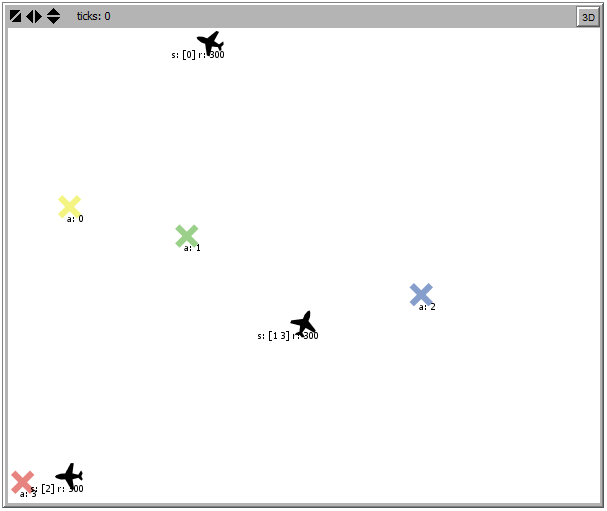
\includegraphics[scale=0.50]{simulation.png}
		\caption{Simulation in the NetLogo}
		\label{fig:simulacao}
	\end{center}
\end{figure}

According to problem formulation (Section \ref{sec:problem}), each task has its location $\langle x,y \rangle$, an associated type of target and the amount of resource required for its execution. The difference in the colors of the tasks represents the different types of targets in Figure \ref{fig:simulacao}, for example, the color red may represent a fire places and the color blue a train of parked vehicles. Each UAV, in addition to its location $\langle x,y \rangle$ and its sensor list, has a ``to-do'' list of tasks. This list starts empty, and when the \uav\ selects a task, it adds the task to this list. 
The ``to-do'' list is a FIFO: the first selected task is the first one to be performed.

The simulation was implemented so that at each tick (simulation time progression unity), all UAVs move one pixel. 
The ticks are used as makespan (total time that elapses from the beginning to the end of the execution). It will never exceed the mission deadline. The execution ends when the \uavs\ complete all tasks they have selected to perform.
It is noteworthy that the makespan (elapsed time) may be easily converted into traveled distance by each UAV since all UAVs move one pixel per tick.

Only one token is released to the \uavs. The token contains the mission tasks and a list of visited agents. This list starts empty and each \uav\ that receives the token adds its ID in the list. At each tick, the token is sent to a random \uav\ that has not yet received the token in the current round, i.e. a \uav\ that is not in the list of visited agents. The token also has a list of unavailable agents. This list is used by the proposed algorithms AL, SAL and LAL (see Section \ref{sec:al}).
When a UAV receives the token, it runs the algorithm to choose the tasks it will perform. 

Several experimental scenarios were created in order to analyze different situations. The scenarios vary in amount of mission tasks, number of agents and size of the area (in pixels) in which they are situated, as listed in the following:

\begin{enumerate}
	\item 3 \uavs; 4 tasks; 300 ticks as deadline; 100 x 80 px area size. \label{case:4tasks}
	\item 3 \uavs; 8 tasks; 300 ticks as deadline; 100 x 80 px area size. \label{case:8tasks}
	\item 3 \uavs; 16 tasks; 300 ticks as deadline; 100 x 80 px area size. \label{case:16tasks}
	\item 3 \uavs; 32 tasks; 300 ticks as deadline; 100 x 80 px area size. \label{case:32tasks}
	\item 6 \uavs; 64 tasks; 300 ticks as deadline; 200 x 160 px area size. \label{case:64tasks}
	\item 9 \uavs; 96 tasks; 300 ticks as deadline; 300 x 240 px area size. \label{case:96tasks}
\end{enumerate}

Each set of \uavs\ -- with 3, 6, and 9 \uavs\ -- were randomly created once. For example, the set of 3 \uavs\ were created once and used in scenarios \ref{case:4tasks}, \ref{case:8tasks}, \ref{case:16tasks}, \ref{case:32tasks}. 
The \uavs' location $\langle x,y \rangle$ were defined randomly, respecting the limit of the scenario's area.
The number of sensors that each \uav\ was equipped as well as the types of sensors were also assigned with random values. Each \uav\ was equipped with one or two sensors of types $s_0$, $s_1$, $s_2$ or $s_3$.

The same was applied for the tasks. The tasks location $\langle x,y \rangle$ and the type of target were defined randomly. 
Each task was assigned a single type of target, which may be of the types $a_0$, $a_1$, $a_2$ or $a_3$.
Only the amount of resources needed to execute a task ($c_j$) was fixed at ten time units (ticks) for all tasks. 

Table \ref{table:quality} presents the sensors' quality to detect each type of target. These values were used in all scenarios. According to this configuration, the target $a_0$, for example, can be detected by the sensors $s_0$ and $s_2$, but with different qualities, while sensors $s_1$ and $s_3$ are unable to detect $a_0$.

\begin{table}[h!]
	\small
	\fontsize{8}{8}\selectfont
	\centering
	\caption{Quality of each sensor to detect the different types of target}
	\label{table:quality}
	\begin{tabular}{|l|c|c|c|c|} \hline
		Sensor / target  & $a_0$  & $a_1$  & $a_2$  & $a_3$    \\ \hline
		$s_0$              & $1.0$  & $0$  & $0.3$  & $0.5$      \\ \hline
		$s_1$              & $0$  & $0$  & $1.0$  & $0$           \\ \hline
		$s_2$              & $0.2$  & $0$  & $0$  & $1.0$        \\ \hline
		$s_3$              & $0$  & $1.0$  & $0$  & $0.3$        \\ \hline
	\end{tabular}
\end{table}


The scenarios were run 30 times for each proposed algorithm. 
In all experiments, the UAVs' capabilities were computed using Equation \ref{eq:capability} with $\alpha = 0.6$, giving higher importance to the distance factor.
Different stimulus values were also tested, but only results with the value 0.6 are shown, as this value presented better results in most cases, as it is known for the Swarm-GAP \citep{ferreira2010robocup}.

The experiments were conducted in a PC with 1.70GHz, 4GB of RAM and SO Windows 8.1 Pro 64 bits. 
The results obtained using the proposed solutions as well as Swarm-GAP are presented and discussed in next section.



\section{Experimental results and analysis}\label{sec:experimental_result}
%In order to evaluate the proposed algorithms, the following metrics were considered:
\begin{inlinelist}
	\item Total reward;
	\item Makespan (total elapsed time from the beginning to the end of the execution);
	\item Quantity of the tasks that were completed; and
	\item Quality of the completed tasks. The main objective is to maximize the total reward (a). Since this metric is influenced by the quantity and quality of the completed tasks (see Section \ref{sec:problem}), the metrics (b), (c) and (d) allow to understand the result of the (a). Furthermore, the
	\item Number of exchanged messages (related to the token-passing mechanism) and the
	\item Algorithm's runtime were also measured and analyzed.
\end{inlinelist}
 
The metrics are applied to evaluate the proposed methods, i.e. AL, SAL and LAL, and compared them to the results obtained using the Swarm-GAP. Part of the achieved results are shown in charts, but the complete data (mean and standard deviation) for all assessed metrics for each algorithm and scenario, from \ref{case:4tasks} to \ref{case:96tasks}, are presented in Tables \ref{table:allresults3uavs} and \ref{table:allresults6or9uavs}. A specific set of scenarios is used to highlight the results for each metric. After their presentation, these results are discussed. At the end of this section, a scalability analysis of the algorithms is provided.

\begin{table}%[h]
	\small
	\fontsize{6}{6}\selectfont
	\centering
	\caption{Total reward, makespan, quantity and quality of the completed tasks, number of exchanged messages and algorithm's runtime for 30 runs of each algorithm in scenarios with 3 \uavs\ and different number of tasks}
	\label{table:allresults3uavs}
	
	\begin{tabular}{rrrrr} \hline
		& Swarm-GAP
		& AL
		& SAL
		& LAL \\ \hline 
		
		& Mean (St.Dev.) & Mean (St.Dev.)  & Mean (St.Dev.)  & Mean (St.Dev.)  \\ [1ex]
		
		\multicolumn{5}{l}{\textbf{3 UAVs and 4 tasks in area of 100x80 pixels with deadline of 300 ticks}} \\
		Total reward           &   1.6971  ($\pm$0.4705) &  2.1016   ($\pm$0.3251)   &  2.0947   ($\pm$0.3579) &   2.2377   ($\pm$0.3217) \\
		Elapsed time (norm)    &   0.3559  ($\pm$0.1874) &  0.431    ($\pm$0.1388)   &  0.4139   ($\pm$0.1486) &   0.3118   ($\pm$0.0759) \\ 
		Comp. tasks (norm)     &   0.7583  ($\pm$0.1796) &  1.0000   ($\pm$0.0000)   &  1.0000   ($\pm$0.0000) &   1.0000   ($\pm$0.0000) \\ 
		Quality (norm)         &   0.8131  ($\pm$0.1784) &  0.8242   ($\pm$0.1284)   &  0.7942   ($\pm$0.1488) &   0.9167   ($\pm$0.1428) \\ 
		%Idle UAVs              &   0.9333  ($\pm$0.5833) &  0.5333   ($\pm$0.5074)   &  0.5667  ($\pm$ 0.504)  &   0.1667  ($\pm$ 0.379) \\ 
		Sending token          &   2.8667  ($\pm$0.3457) &  4.2000   ($\pm$1.7889)   &  4.0333   ($\pm$1.7317) &   6.9667   ($\pm$2.2816) \\ 
		%Cost = (t + me) / ct   &   36.1433               &  33.3750                &   32.0500             &  25.1250        \\ 
		Total Runtime (sec)    &   2.1047  ($\pm$1.5154) &  2.6855   ($\pm$2.1459)   &  3.4192   ($\pm$3.5977) &   3.9216   ($\pm$2.9873) \\ [1ex]
		%Runtime each run       &   0                     &        0      0         &  0            0       &   0            0 \\ 
		
		\multicolumn{5}{l}{\textbf{3 UAVs and 8 tasks in area of 100x80 pixels with deadline of 300 ticks}} \\
		Total reward           &    2.9436 ($\pm$0.4874)   &  3.651   ($\pm$0.2064)   &  3.6006  ($\pm$0.3246) &   4.8462  ($\pm$1.3581) \\
		Elapsed time (norm)    &   0.6881  ($\pm$0.1722)   &  0.7731  ($\pm$0.1103)   &  0.7382  ($\pm$0.1264) &   0.6786  ($\pm$0.0676) \\ 
		Comp. tasks (norm)     &   0.7708  ($\pm$0.1316)   &  0.9958  ($\pm$0.0228)   &  0.9833  ($\pm$0.0432) &   1.0000  ($\pm$0.0000) \\ 
		Quality (norm)         &   0.7502  ($\pm$0.1599)   &  0.7699  ($\pm$0.0892)   &  0.7273  ($\pm$0.1003) &   0.8125  ($\pm$0.1247) \\ 
		%Idle UAVs              &  0.3000   ($\pm$0.4661)   &  0.1667  ($\pm$0.3790)   &  0.2000  ($\pm$0.4068) &   0.0000  ($\pm$0.0000) \\ 
		Sending token          &   2.9667  ($\pm$0.1826)   &  6.8000  ($\pm$2.6182)   &  6.0000  ($\pm$2.3781) &   11.1667 ($\pm$2.3057) \\ 
		%Cost = (t + me) / ct   &   33.9566       0         &  29.9664                 &  28.9151               &   26.8417               \\ 
		Total Runtime (sec)    &  2.0803   ($\pm$0.6082)   &  2.7879  ($\pm$0.8128)   &  3.4072  ($\pm$1.3381) &   4.8462  ($\pm$1.3581) \\ [1ex]
		
		\multicolumn{5}{l}{\textbf{3 UAVs and 16 tasks in area of 100x80 pixels with deadline of 300 ticks}} \\
		Total reward           &   6.6424  ($\pm$1.0648)    &  7.6047  ($\pm$0.8502)  &  8.7607  ($\pm$0.6316) &   10.5753 ($\pm$0.4666) \\
		Elapsed time (norm)    &   0.9179  ($\pm$0.0495)    &  0.9462  ($\pm$0.0354)  &  0.9210  ($\pm$0.0496) &   0.9027  ($\pm$0.0599) \\ 
		Comp. tasks (norm)     &   0.7229  ($\pm$0.0815)    &  0.8604  ($\pm$0.0585)  &  0.9313  ($\pm$0.0474) &   0.9896  ($\pm$0.0288) \\ 
		Quality (norm)         &   0.8110  ($\pm$0.1040)    &  0.7431  ($\pm$0.0990)  &  0.7849  ($\pm$0.0591) &   0.9239  ($\pm$0.0588) \\ 
		%Idle UAVs              &   0.0333  ($\pm$0.1826)    &  0.0000  ($\pm$0.0000)  &  0.0000  ($\pm$0.0000) &   0.0000  ($\pm$0.0000) \\ 
		Sending token          &   3.0000  ($\pm$0.0000)    &  5.7333  ($\pm$2.5316)  &  6.3667  ($\pm$1.4259) &   18.7667 ($\pm$1.9420) \\ 
		%Cost = (t + me) / ct   &   24.0662                  &  21.0363                &  18.9709               &   18.2885               \\ 
		Total Runtime (sec)    &   2.6142  ($\pm$0.8415)    &  2.8474  ($\pm$1.0097)  &  3.2888  ($\pm$0.9664) &   6.7701  ($\pm$2.5940) \\ [1ex]
                                                                                                                              
		\multicolumn{5}{l}{\textbf{3 UAVs and 32 tasks in area of 100x80 pixels with deadline of 300 ticks}} \\
		Total reward           &   9.1017  ($\pm$1.4553)   &  9.0073  ($\pm$1.2457)    &  13.7469 ($\pm$0.8765) &   19.9057  ($\pm$0.4189) \\
		Elapsed time (norm)    &   0.9624  ($\pm$0.0177)   &  0.9652  ($\pm$0.0185)    &  0.9554  ($\pm$0.0168) &   0.9422   ($\pm$0.0186) \\ 
		Comp. tasks (norm)     &   0.4781  ($\pm$0.0533)   &  0.4844  ($\pm$0.0498)    &  0.6094  ($\pm$0.0391) &   0.7604   ($\pm$0.0222) \\ 
		Quality (norm)         &   0.7416  ($\pm$0.0723)   &  0.7275  ($\pm$0.0910)    &  0.8741  ($\pm$0.0512) &   0.9315   ($\pm$0.0292) \\ 
		%Idle UAVs              &   0.0000  ($\pm$0.0000)   &  0.0000  ($\pm$0.0000)    &  0.0000  ($\pm$0.0000) &   0.0000   ($\pm$0.0000) \\ 
		Sending token          &   3.0000  ($\pm$0.0000)   &  3.5333  ($\pm$0.8996)    &  3.8333  ($\pm$0.9129) &   24.8000  ($\pm$1.4716) \\ 
		%Cost = (t + me) / ct   &   19.0675                 &  18.9097                  &  14.8957               &   12.6356                \\ 
		Total Runtime (sec)    &   2.9778  ($\pm$0.7843)   &  3.2434  ($\pm$1.1824)    &  4.0268  ($\pm$1.0639) &   10.9934  ($\pm$2.1070) \\ [1ex]
                     
		\hline
	\end{tabular}
\end{table} 

\begin{table}%[ht]
	\small
	\fontsize{6}{6}\selectfont
	\centering
	\caption{Total reward, makespan, quantity and quality of the completed tasks, number of exchanged messages and algorithm's runtime of 30 runs of each algorithm in scenarios with different number of \uavs\ and tasks}
	\label{table:allresults6or9uavs}
	
	\begin{tabular}{rrrrr} \hline
		& Swarm-GAP
		& AL
		& SAL
		& LAL \\ \hline 
		
		& Mean (St.Dev.) & Mean (St.Dev.)  & Mean (St.Dev.)  & Mean (St.Dev.)  \\ [1ex]
		
		\multicolumn{5}{l}{\textbf{6 UAVs and 64 tasks in area of 200x160 pixels with deadline of 300 ticks}} \\
	Total reward           &    12.1152 ($\pm$1.9136)  & 12.9234 ($\pm$1.8407)  & 28.2929 ($\pm$1.0694) & 38.7922  ($\pm$1.2800)  \\
	Elapsed time (norm)    &    0.9850  ($\pm$0.0086)  & 0.9819  ($\pm$0.0100)  & 0.9737  ($\pm$0.0101) &  0.9643  ($\pm$0.0116)  \\ 
	Comp. tasks (norm)     &    0.3135  ($\pm$0.0323)  & 0.3302  ($\pm$0.0317)  & 0.5271  ($\pm$0.0201) &  0.6813  ($\pm$0.0208)  \\ 
	Quality (norm)         &    0.7358  ($\pm$0.0790)  & 0.7447  ($\pm$0.0689)  & 0.9582  ($\pm$0.0319) &  0.9667  ($\pm$0.0165)  \\ 
	%Idle UAVs              &    0.0000  ($\pm$0.0000)  & 0.0000  ($\pm$0.0000)  & 0.0000  ($\pm$0.0000) &  0.0000  ($\pm$0.0000)  \\ 
	Sending token          &    6.0000  ($\pm$0.0000)  & 6.5333  ($\pm$0.9371)  & 6.6333  ($\pm$1.0334) &  44.0000 ($\pm$1.5086)  \\ 
	%Cost = (t + me) / ct   &  15.0249                  & 14.2477                &  8.8557               &  7.6445                 \\ 
	Total Runtime (sec)    &    7.2348  ($\pm$3.4657)  & 10.7935 ($\pm$5.7570)  &  9.7962 ($\pm$4.7782) &  31.9513 ($\pm$8.3246)  \\ [1ex]

		\multicolumn{5}{l}{\textbf{9 UAVs and 96 tasks in area of 300x240 pixels with deadline of 300 ticks}} \\
	Total reward           &  15.582  ($\pm$2.0050) & 16.724   ($\pm$2.1908)  & 37.9608  ($\pm$1.1119) & 44.733  ($\pm$1.5961)   \\
	Elapsed time (norm)    &  0.9886  ($\pm$0.0082) & 0.9894   ($\pm$0.0064)  &  0.9763  ($\pm$0.0092) & 0.9693  ($\pm$0.0124)    \\ 
	Comp. tasks (norm)     &  0.2611  ($\pm$0.0217) & 0.2774   ($\pm$0.0276)  &  0.4674  ($\pm$0.0170) & 0.5226  ($\pm$0.0162)    \\ 
	Quality (norm)         &  0.7899  ($\pm$0.0599) & 0.7865   ($\pm$0.0641)  &  0.9680  ($\pm$0.0202) & 0.9752  ($\pm$0.0159)   \\ 
	%Idle UAVs              &  0.0000  ($\pm$0.0000) &   0.0000 ($\pm$0.0000)  &  0.0000  ($\pm$0.0000) &  0.0000 ($\pm$0.0000)   \\ 
	Sending token          &  9.0000  ($\pm$0.0000) &  9.8667  ($\pm$1.1958)  &  9.7000  ($\pm$1.2360) &  51.500 ($\pm$1.4797)   \\ 
	%Cost = (t + me) / ct   &  12.1901               &  11.5157                &  6.7444                &  6.8233                \\ 
	Total Runtime (sec)    &  9.0990  ($\pm$4.6221) &  13.1253 ($\pm$7.6605)  & 12.2062  ($\pm$2.7515) & 50.5544 ($\pm$31.2161)   \\ [1ex]
		
		\hline
	\end{tabular}
\end{table} 

Scenarios \ref{case:4tasks}, \ref{case:8tasks}, \ref{case:16tasks} and \ref{case:32tasks}, which are composed of 4, 8, 16 and 32 tasks, respectively, are used to demonstrate the results of the total reward, makespan, quantity and quality of the completed tasks and number of exchanged messages. These four scenarios were selected due to the fact that they have the same number of \uavs\ and the amount of tasks is varied, but with the same mission's deadline. This choice allows to evaluate situations in which the UAVs have enough time, or more than enough, to perform the tasks (this is the case for scenarios \ref{case:4tasks} and \ref{case:8tasks}), and situations in which the UAVs have a short time to perform a large number of tasks (scenarios \ref{case:16tasks} and \ref{case:32tasks}).  In the former, the UAVs can perform all tasks, but they must do it in the shortest time. On the other hand, in the second situation the UAVs do not have enough time to perform all tasks. Then, they must perform as many tasks as possible.

\subsection{Total reward}

The total reward of each method for the different scenarios is shown in Figure \ref{grafico:total_capability}. In scenarios with 4 and 8 tasks, both AL and SAL algorithms outperformed the Swarm-GAP by about 24\%.

As the amount of tasks increases, SAL allows a greater total reward than AL. SAL outperformed Swarm-GAP by 31.89\% and 51.03\% in the scenarios with 16 and 32 tasks, respectively, while AL overcomes the Swarm-gap by 14.48\% in scenario with 16 tasks. AL and Swarm-GAP presented the same results in the scenario with 32 tasks.

The highest total reward was obtained by the LAL algorithm. This variant outperformed Swarm-GAP by 31.85\%, 64.63\%, 59.2\% and 118.7\% in the scenarios with 4, 8, 16 and 32 tasks, respectively. This pattern of enhancement in the total reward can also be observed in the scenario with 64 and 96 tasks (See table \ref{table:allresults6or9uavs}). The LAL algorithm presented results 3.2 and 2.87 times better than Swarm-GAP.

%\input{graficos/total_capability}
\begin{figure}[h]
	\begin{center}
		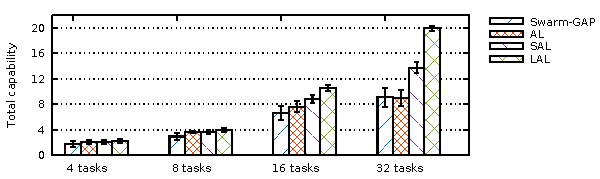
\includegraphics[scale=1.00]{total_capability.pdf}
		\caption{Total reward of each method for different scenarios with stimulus 0.6}
		\label{grafico:total_capability}
	\end{center}
\end{figure}

\subsection{Makespan and quantity of completed tasks}

The quantity of completed tasks for each algorithm in each scenario is presented in Figure \ref{grafico:tarefasconcluidas}. 
The results presented in this figure are normalized by the number of tasks of each scenario. Figure \ref{grafico:ticks} shows the elapsed time (in ticks), normalized by the deadline associated to the mission. 
As it is possible to observe, using time efficiently, the \uavs\ can perform more tasks achieving greater total rewards.

%\input{graficos/graficos_completed_tasks}
\begin{figure}[h]
	\begin{center}
		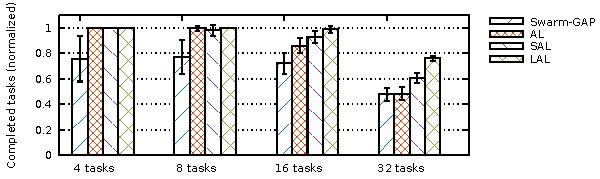
\includegraphics[scale=1.00]{completed_tasks.pdf}
		\caption{Completed tasks of each method for different scenarios with stimulus 0.6}
		\label{grafico:tarefasconcluidas}
	\end{center}
\end{figure}


%\input{graficos/graficos_ticks}
\begin{figure}[h]
	\begin{center}
		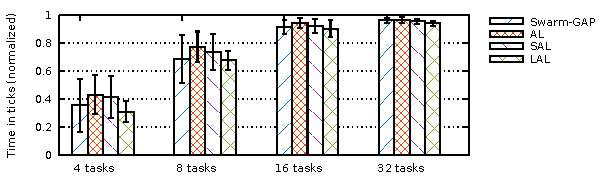
\includegraphics[scale=1.00]{makespan.pdf}
		\caption{Makespan of each method for different scenarios with stimulus 0.6}
		\label{grafico:ticks}
	\end{center}
\end{figure}

In scenarios with 4 and 8 tasks, in which there is enough time (extended or relaxed deadline) for the UAVs carrying out all the tasks (the whole mission), the Swarm-GAP algorithm results in \uavs\ not using all the available resources. In these cases they have used only 35.59\% and 68.81\% of the time. Moreover, more than 22\% of the tasks were not performed in these two scenarios. The slack time (65\% and 32\%, respectively, in scenarios with 4 and 8 tasks) could have been used to perform other tasks. On the other hand, using Allocation Loop (AL) method allowed 100\% and 99\% of the tasks to be performed. This was possible because while a \uav\ still has resources, it may select more tasks to perform in this method.

When the algorithms with Sorting and Allocation Loop (SAL), and Limit and Allocation Loop (LAL) were used, the \uavs\ have also performed all tasks in scenarios with 4 and 8 tasks. However, they took less time than the AL. The LAL, for instance, improves the elapsed time by 27\% and 12\% compared to AL in the scenarios with 4 and 8 tasks, respectively.

In scenarios with 16 and 32 tasks, i.e., those in which there are more tasks to be performed, the use of the SAL algorithm causes more tasks to be performed, in comparison to Swarm-GAP and AL, without increasing the elapsed time. For instance, in the scenario with 16 tasks, the use of SAL increased the amount of completed tasks by 28.8\% compared to Swarm-GAP. The LAL method improves this performance even further. 
In the scenario with 16 tasks, it happened simulation runs in which the UAVs have performed all tasks when using the LAL algorithm. Furthermore, in the scenario with 32 tasks, LAL increased the completed tasks by 59\%, whereas still reducing the elapsed time by 2.09\% compared to Swarm-GAP.

\subsection{Quality of completed tasks}

The average quality of the completed tasks in each scenario is shown in Figure \ref{grafico:qualidade}. The quality metric was normalized in relation to the number of completed tasks. The higher the quality of the tasks performed by the agents, the greater the total reward. For this measure, the LAL algorithm also shown the best results.

%\input{graficos/graficos_quality}
\begin{figure}[h!]
	\begin{center}
		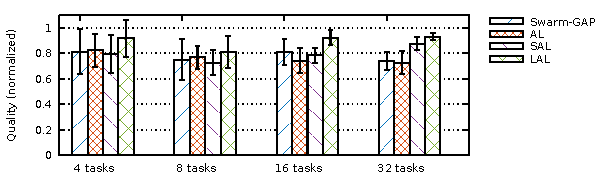
\includegraphics[scale=1.00]{quality.pdf}
		\caption{Quality of each method for different scenarios with stimulus 0.6}
		\label{grafico:qualidade}
	\end{center}
\end{figure}

In the scenarios with 4 and 8 tasks, the methods Swarm-GAP, AL, and SAL presented similar results in the quality of the completed tasks. However, Swarm-GAP outperformed SAL, but only in about 3\%. LAL increased by 12.74\% and 8.3\% the quality of the completed tasks in the scenario with 4 and 8 tasks, respectively, compared to the Swarm-GAP algorithm. 

In the scenario with 16 tasks, SAL still has a slightly lower result than Swarm-GAP (-3.2\%). However, when there are more tasks, such as in the scenario with 32 tasks, SAL improved the quality by 17.86\% compared to the Swarm-GAP. In the scenarios with 16 and 32 tasks, LAL presents an improvement of 13.92\% and 25.6\% compared to the Swarm-GAP, respectively. This pattern of quality improvement can also be observed in the other experiments 
with 64 and 96 tasks (see Table \ref{table:allresults6or9uavs}).

\subsection{Number of exchanged messages}

Figure \ref{grafico:trocamensagens} shows the number of exchanged messages for each algorithm in each scenario.
It is possible to notice that this number is nearly constant in the Swarm-GAP, AL and SAL, while in the LAL method the number of exchanged messages increases linearly with the amount of completed tasks. 
The behavior of  the three first algorithms is due to the fact that in these algorithms the number of the tokens that are sent relates more to the amount of agents than to the number of performed tasks.

%\input{graficos/graficos_msg}
\begin{figure}[h!]
	\begin{center}
		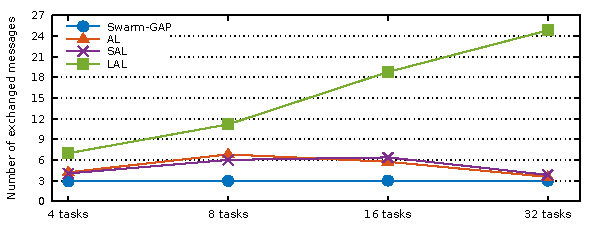
\includegraphics[scale=1.00]{exchanged_messages.pdf}
		\caption{Total number of exchanged messages of each method for different scenarios  with stimulus 0.6}
		\label{grafico:trocamensagens}
	\end{center}
\end{figure}

Using Swarm-GAP, each UAV receives the token at most once. When the UAV does not receive it, this means that all tasks were already selected before the token arrives to this given UAV. Anyway, when there is a given number of agents, for example three, the token is sent three times and then it is discarded. For AL and SAL, each \uav\ can receive the token more than once. On average, each \uav\ receives approximately one to two times the token.
Due to LAL's limitation of choosing at most one task at a time that the \uav\ receives the token, 
the number of exchanged messages is about the same number of performed tasks.

Despite the higher number of exchanged messages in the LAL algorithm, the quantity of completed tasks improved and the elapsed time decreased. Hence, the LAL algorithm enables \uavs\ to spend less time in the execution of each task, i.e., the cost to carry out the tasks decreases.

In order to investigate if this increase in the number of exchanged messages is rewarded by the quantity of completed tasks, Figure \ref{grafico:custoportarefa} presents the average cost to perform each task, considering also the number of exchanged messages. 
Then, the cost was computed by $avgcost = (t + em) / ct$, where ($t$) is the elapsed time, ($em$) is number of exchanged messages and ($ct$) is the amount of completed tasks.

%\input{graficos/graficos_custo}
\begin{figure}[h!]
	\begin{center}
		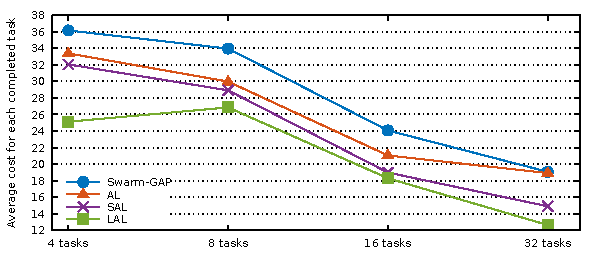
\includegraphics[scale=1.00]{avgcost.pdf}
		\caption{Average cost of the completed tasks (considering number of exchanged messages) of each method for different scenarios  with stimulus 0.6}
		\label{grafico:custoportarefa}
	\end{center}
\end{figure}

Even assuming that the amount of exchanged messages is also considered in the cost of executing the tasks, the LAL algorithm still reduces it compared to Swarm-GAP, by 30.48\%, 20.95\%, 24\% and 33.73\%, respectively for the scenarios with 4, 8, 16 and 32 tasks. 
 

\subsection{Algorithm's Runtime} \label{sec:runtime}

The scenarios \ref{case:32tasks}, \ref{case:64tasks} and \ref{case:96tasks}, which are composed of 32, 64, and 96 tasks, respectively, are used to illustrate the runtime results for the proposed algorithms.
The amount of \uavs\ in these scenarios is varied, and the number of tasks is greater. The runtime was measured in seconds, using the NetLogo profiler extension. 

The results of 30 runs (mean and standard deviation) of these scenarios, with all considered metrics (see Section \ref{sec:experimental_result}), can be seen in the Tables \ref{table:allresults3uavs} and \ref{table:allresults6or9uavs}. 
Here, the runtime analysis of each algorithm in different scenarios is highlighted in the Table \ref{table:runtime}.
This table shows the mean total runtime in seconds, 
the number of times the algorithm was executed and the mean runtime of each execution.
It is worth to notice that the number of times the algorithm was executed is the same of the number of exchanged messages.

\begin{table}[ht]
	\small
	\fontsize{8}{8}\selectfont
	\centering
	\caption{Runtime analysis of each method (in seconds) in different scenarios}
	\label{table:runtime}
	
	\begin{tabular}{clrrrr} \hline
		Scenario   &                               & Swarm-GAP &  AL     & SAL     & LAL    \\ \hline 
		32 tasks   & Total runtime (mean) in sec.  & 2.9778 & 3.2434 & 4.0268 & 10.9934 \\ 
		3 UAVs     & Execution times (mean)        & 3.0000 & 3.5333 & 3.8333 & 24.8000 \\ 
		           & Seconds per run               & 0.9926 & 0.9179 & 1.0504 & 0.4432  \\ [1ex]
		64 tasks   & Total runtime (mean) in sec.  & 7.2348 & 10.7935 & 9.7962 & 31.9513 \\ 
		6 UAVs     & Execution times (mean)        & 6.0000 & 6.5333  & 6.6333 & 44.0000 \\ 
				   & Seconds per run               & 1.2058 & 1.6520  & 1.4768 & 0.7261  \\ [1ex]
		96 tasks   & Total runtime (mean) in sec.  & 9.0990  & 13.1253 & 12.2062 & 50.5544 \\ 
		9 UAVs     & Execution times (mean)        & 9.0000  & 9.8667  & 9.7000  & 51.5000 \\ 
		           & Seconds per run               & 1.0110  & 1.3302  & 1.2583  & 0.9816  \\ [1ex] \hline 
	\end{tabular}
\end{table} 

The total runtime for AL and SAL are almost the same for each scenario. This suggests that sorting the tasks in SAL algorithm has not a great impact in the runtime. 
The AL and SAL results are close to Swarm-GAP in the scenario with 32 tasks. 
However, in the scenarios with 64 and 96 tasks, the availability check, that avoids the token remain in the network forever, impacts the runtime due to the greater number of tasks. 
For instance, the AL total runtime increases by 44.24\% compared to Swarm-GAP in the scenario with 96 tasks.

On the other hand, the LAL increases the total runtime for all scenarios compared to the others algorithms.
Due to the limit to select tasks, the LAL algorithm is executed more times causing the total runtime to increase. 
For example, in the scenario with 96 tasks, the LAL algorithm was executed on average 51.5 times -- that is the same number of exchanged messages. 
Although the LAL presented a high total runtime, each \uav\ took 0.9816 seconds, on average, to execute the algorithm each time it received the token in this scenario with 96 tasks.

\subsection{Discussions} \label{sec:discussion}
This section aims to identify the main aspects found during the replications done and to analyze all obtained results (see Section \ref{sec:findings}), identifying its implications for practice (see Section \ref{sec:implications}), characterizing the threats to the study validity (see Section \ref{sec:threats}), listing the main existing limitations in this work done and the opportunities to perform further investigations based on this one (see Section \ref{sec:limitations}).

\subsection{Scalability analysis} \label{sec:scalability}
In order to test the scalability of the proposed solutions, two new experimental scenarios were created. 
They have a very large number of agents and tasks (100 \uavs\ and 500 tasks) and differ from each other by the missions' deadline. These two additional scenarios are described as follows:

\begin{enumerate}
	\setcounter{enumi}{6}
	\item 100 \uavs; 500 tasks; 300 ticks as deadline; 750 x 750 px area size. \label{case:500tasks300deadline}
	\item 100 \uavs; 500 tasks; 1000 ticks as deadline; 750 x 750 px area size. \label{case:500tasks1000deadline}
\end{enumerate}

It is worth mentioning that the quantities used in these scenarios extrapolate those that would be expected in a real situation. However, the intention here is to stress these numbers to discuss scalability. 
The results (total reward, makespan, quantity and quality of completed tasks and number of exchanged messages) of 30 runs are shown in Table \ref{table:500tasks}.

\begin{table}%[t]
	\small
	\fontsize{6}{6}\selectfont
	\centering
	\caption{Total reward, makespan, quantity and quality of completed tasks and number of exchanged messages of 30 runs of each algorithm in scenarios with 100 \uavs\ and 500 tasks}
	\label{table:500tasks}
	
	\begin{tabular}{rrrrr} \hline
		& Swarm-GAP
		& AL
		& SAL
		& LAL \\ \hline 
		
		& Mean (St.Dev.) & Mean (St.Dev.)  & Mean (St.Dev.)  & Mean (St.Dev.)  \\ [1ex]
		
		\multicolumn{5}{l}{\textbf{100 UAVs and 500 tasks in area of 750x750 pixels with deadline of 300 ticks}} \\
		Total reward           &  162.0141  ($\pm$6.5974) &  162.9333  ($\pm$7.0324)   &  339.2015  ($\pm$7.5146)  &  240.956   ($\pm$3.6869)   \\
		Elapsed time (norm)    &  0.9979    ($\pm$0.0020) &  0.9978    ($\pm$0.0020)   &  0.9908    ($\pm$0.0029)  &  0.9992    ($\pm$0.0023)   \\ 
		Comp. tasks (norm)     &  0.4063    ($\pm$0.0141) &  0.4090    ($\pm$0.0161)   &  0.7269    ($\pm$0.0159)  &  0.5022    ($\pm$0.0075)   \\ 
		Quality (norm)         &  0.7789    ($\pm$0.0234) &  0.7736    ($\pm$0.0190)   &  0.9638    ($\pm$0.0085)  &  0.9707    ($\pm$0.0078)   \\ 
		%Idle UAVs              &  0.0000    ($\pm$0.0000) &  0.0000    ($\pm$0.0000)   &  0.4333    ($\pm$0.5683)  &  0.0000    ($\pm$0.0000)   \\ 
		Sending token          &  100       ($\pm$0.0000) &  103.4667  ($\pm$1.9070)   &  104.5333  ($\pm$1.8889)  &  298.1333  ($\pm$2.5695)   \\ 
		%Cost = (t + me) / ct   & 1.9660                  &  1.9697                   &  1.1055                  &  2.3811                   \\ 
		%Total Runtime (sec)    & 335.1766   ($\pm$92.466) &  550.796   ($\pm$261.7752) &  1164.9918 ($\pm$343.6324) &  2163.343 ($\pm$287.6923)  \\ 
		[1ex]	\hline
		
		\multicolumn{5}{l}{\textbf{100 UAVs and 500 tasks in area of 750x750 pixels with deadline of 1000 ticks}} \\
		Total reward           &  227.1356  ($\pm$8.4193)    &  230.5901  ($\pm$9.4936) &  435.3937 ($\pm$5.3410)    &  461.5992  ($\pm$2.0479)  \\
		Comp. tasks (norm)     &  0.7295    ($\pm$0.0213)    &  0.7420    ($\pm$0.0230) &  1.0000   ($\pm$0.0000)    &  1.0000    ($\pm$0.0000) \\ 
		Elapsed time (norm)    &  0.9983    ($\pm$8.0E-4)    &  0.9982    ($\pm$8.0E-4) &  0.9925   ($\pm$0.0028)    &  0.9856    ($\pm$0.0123)  \\ 
		Quality (norm)         &  0.7960    ($\pm$0.0173)    &  0.7902    ($\pm$0.0154) &  0.9650   ($\pm$0.0138)    &  0.9778    ($\pm$0.0058) \\ 
		%Idle UAVs              &  0.0000    ($\pm$0.0000)    &  0.0000    ($\pm$0.0000) &  38.7333  ($\pm$2.6773)    &  0.0000    ($\pm$0.0000)   \\ 
		Sending token          &  100       ($\pm$0.0000)    &  110.1667  ($\pm$2.6141) &  65.7667  ($\pm$4.2966)    &  526.1667  ($\pm$12.3821)  \\ 
		%Cost = (t + me) / ct   &  3.0111                    & 2.9875                  &  2.1165                   &  3.0235                   \\ 
		%Total Runtime (sec)    &  244.3903  ($\pm$30.1872)   & 356.2328   ($\pm$25.864) &  404.3574 ($\pm$343.8118)  &  2879.1853 ($\pm$567.0917)  \\ 
		[1ex]	\hline
	\end{tabular}
\end{table} 

The AL algorithm presented similar results to Swarm-GAP, in both scenarios (\ref{case:500tasks300deadline} and \ref{case:500tasks1000deadline}).
SAL had an increase of around 100\% in the total reward, compared to Swarm-GAP, in both scenarios.
LAL also outperformed Swarm-GAP in both scenarios. 
The total reward had an improvement of 48.72\% and 103.22\% when LAL is used, compared to Swarm-GAP, respectively in scenarios \ref{case:500tasks300deadline} and \ref{case:500tasks1000deadline}.

Although the LAL method presents the best results in most of the performed experiments, it was overcome by SAL in scenario \ref{case:500tasks300deadline}.
Due to the limit of selection imposed by the LAL, each \uav\ can select no more than 3 tasks in total. This is because the deadline is 300 ticks and there are 100 \uavs\ (at each tick one \uav\ receives the token). Thus, always less than 300 tasks will be performed, even if there are 500 tasks to be performed.
On the other hand, in the scenario \ref{case:500tasks1000deadline}, in which there is a large time window to the \uavs\ perform the tasks (1000 ticks of deadline), LAL is the best in terms of total reward.

% Colocar na tabela: seconds per run??




\section{Related work}\label{sec:rw}
%The works presented by \textit{Alighanbari and How}\cite{alighanbari2005decentralized} and \textit{Schwarzrock et al.}\cite{MAS07} provide the task assignment for a fleet of UAVs, having a decentralized structure with no central command, and running only in static context. The algorithms presented by them were not tested in scenarios were changes can occur during the execution, e.g., the number of agents or tasks changes while the mission is being performed. However, both works mentioned a necessity of reassign tasks in case of any scenario parameter change, leaving an idea to future work. This idea was used in our study to suggest a token reset by the algorithm.

Our work presents a proposal inspired in what was shown by \textit{Schwarzrock et al.}\cite{MAS07} and topics related with tasks allocation and Multi-Agent Systems(MAS) presented by other authors \cite{MAS01, MAS02, MAS03, MAS04, MAS05, MAS06}, extending applied concepts to dynamic context. Although there are centralized solutions to this problem, such as what was presented by \textit{Jose and Pratihar}\cite{jose2016task}, that uses genetic algorithm to assign tasks to a set of robots in a inspection system, this kind of solution is not suitable to the present work because in our scenario there is no guarantee of communication among all elements.

Multiobjective Optimization Problems (MOP) are represented by a vector of decisions satisfying some constraints and aim to optimize a vector of functions that represents an objective. The number of constraints must be less or equals to the number of elements in decision vector, otherwise it is created a problem called as over-constrained. In this scenario, as shown by Coello et al.\cite{MOEA01},  multiobjective evolutionary algorithms (MOEA) appear as a powerful tool to analyze all objectives and their constraints, maximizing global results. This optimization is done with rounds of data analysis trying to converge to the better response. Zitzler et al.\cite{07} compared some approaches to solve MOP and it is possible to identify a common characteristic in the communication protocol that defines a way to redistribute the functions aiming to optimize results. We used this strategy applying more than one communication round in the extended algorithms here proposed.

Ferreira et al. \cite{ferreira2007swarm} provided evidence that the $stimulus$ value of $0.6$ generates best results when applied to calculate the capability of task execution by the agent. However, that analysis was done based on a static scenario. Our work identified a slight difference of $\simeq 3\%$ in results when applied different $stimulus$ in dynamic context. For a fair comparison with the original study \cite{MAS07} and considering the small difference in results, we adopted the value of $0.6$ for this variable.

Many works \cite{ferreira2007swarm,scerri2005allocatingLADCOP, ferreira2010robocup,ikemoto2010adaptive} deal with the allocation task problem. In those studies, the organization and tasks ordering are done by a central command unit. However, this strategy generates a huge amount of messages to transmit the tasks and it can cause a network overhead. To deal with this, the strategy adopted by \textit{Schwarzrock et al.}\cite{MAS07} was the Swarm-GAP, so that it is easier to add agents in the structure or even to treat sensors onboard issues. Our work follows the same strategy based on the requirement of decentralized structure of decision using swarm intelligence.

\section{Conclusion} \label{sec:conclusions}
%Since the original work \cite{MAS07} is classified as a reproducible research\cite{exp02} and confirmed by the reproduction displayed in Section \ref{sec:background}, we performed two independent replications, using NetLogo 5.3.1 environment, to collect results and obtain evidences about limitations and improvements opportunities proposed by the present study.

With an approaching closer to real world, we defined a dynamic context in substitution of the original static one used in \cite{MAS07}, and performed a first replication to validate that the original algorithms proposed by \textit{Schwarzrock et al.} are fully functional in this new dynamic scenario. This experiment showed an improvement opportunity due to a decrease in some dependent variables, e.g., capability and quality. 

Proceeding an action research and based on results obtained by the original work, we proposed extended algorithms to better address the new dynamic scenario created. The second replication, assessed these extended algorithms and permitted to identify and discuss emerging trade-offs. The variables quality and exchanged messages were the focus of these analysis due to the variance presented by the extended algorithms in these variables compared with the original ones.

The proposal here presented has, as the main idea, all tasks releasing after the team loose an agent, and the token resetting to permit a new turn of allocation execution steps. Thus, the tasks not completed can be reallocated always looking for the quality maximization based on the relation among the task distance and the sensor suitability to its realization. There are evidences that this new procedure execution requires more communication since the number of exchanged messages increased more than 100\%.

The main discussion is the collateral effect caused to obtain a quality increasing. This effect is an increase in the exchanged messages that suggested some idea of network requirement level to apply the algorithms proposed. However, this measure of network level requirements is left as suggestion of future work. Furthermore, the communication structure used, initially a ring network, can impact in results and different typologies can be tested in the future.


\section*{References}
\bibliographystyle{elsarticle-num}
\bibliography{references}

\end{document}